\documentclass[a4paper]{article}
\usepackage[T1]{fontenc}

\usepackage[left=2cm,right=2cm,top=2.5cm,bottom=2.5cm]{geometry}
\usepackage{hyperref}
\usepackage{csquotes}
\usepackage{parskip}
\usepackage{titlesec}
\usepackage{enumitem}
\usepackage{caption}
\usepackage[swedish]{babel}
\usepackage{fancyhdr}
\usepackage{graphicx}
\usepackage{framed}
\usepackage{pdfpages}

\titleformat{\section}{\large\bfseries}{}{0.0em}{}
\titleformat{\subsection}{\normalsize\bfseries}{}{0.0em}{}

\newenvironment{quotationb}%
{\begin{leftbar}}%
{\end{leftbar}}

\begin{document}

\pagestyle{fancy}
\lhead{
\includegraphics[height=4em]{lithekod.png}}
\rhead{Vårmöte 2022\\Linköping 2022--05--10\\\phantom{}}
\pagenumbering{gobble}

\setlength{\headheight}{50pt}

\begin{center}
{\huge LiTHe kod vårmöte 2022}\par
\vspace{0.5em}
{\Large Ada Lovelace}\par
{2022--05--10}
\vspace{1.5em}
\end{center}

\section{Mötets öppnande}

Mötet öppnas 18:15 av Gustav Sörnäs.

\section{Val av mötesordförande}

Gustav nominerar Victor Lells.

Mötet beslutar att välja Victor Lells till mötesordförande.

\section{Val av mötessekreterare}

Victor nominerar Gustav.

Mötet beslutar att välja Gustav Sörnäs till mötessekreterare.

\section{Val av justeringsperson tillika rösträknare}

Victor nominerar Lowe Kozak och Frans Skarman.

Mötet beslutar att välja Lowe Kozak och Frans Skarman till justeringsperson tillika
rösträknare.

\section{Fastställande av röstlängden}

Mötet beslutar att fastställa röstlängden till 8.

\section{Beslut om mötets stadgeenliga utlysande}

Mötet beslutar att mötet var stadgeenligt utlyst.

\section{Styrelsens verksamhetsberättelse}

Gustav läser upp verksamhetsberättelsen för verksamhetsåret 21/22.

\begin{quotationb}

Verksamhetsåret började med en stor osäkerhet kring COVID. Efter en stund kom vi
    igång och numera har vi även styrelsemöten på plats. Om inte allt går helt
    sidleds under sommaren ser vi fram emot ett helt verksamhetsår på plats
    nästa år.

På inbjudan av Köpenhamns universitet skickade vi två lag till Danmark under
    NWERC. sigma bools placerade sig på 97:e plats med 3 lösta problem. Nästa år
    ser vi fram emot att skicka iväg några lag ut i Europa.

Admin-mässigt har vi rensat databasen på inaktiva medlemmar. Numera har vi 93
    aktiva medlemmar. Anekdotiskt har vi sett några nya ansikten, och den
    föreslagna styrelsen är till och med fler nya än gamla!

På höstmötet fick styrelsen i uppdrag att se över protokollföringen så att den
    följer GDPR. Resultatet av arbetet presenteras i form av en proposition
    senare under mötet.

På game jam-fronten gick Fall game jam på plats med bra närvaro i Ebbepark efter
    att Creactive fortsatt inte öppnat. Kanske kommer vi kunna återvända dit i
    höst efter att Internetstiftelsen tagit över. Tagga tagga! Global game jam
    gick på distans med närvaron som hör till det, och Spring har i skrivande
    stund inte skett. Game jam-gruppen testade att stå i Collo (föreningens
    första?) med oklara resultat. Folk hade kul så det kommer nog fortsatt ske.

\end{quotationb}

\section{Styrelsens ekonomiska berättelse}

Victor läser upp den ekonomiska berättelsen för verksamhetsåret 21/22.

\begin{quotationb}

\textbf{Utgångspunkt 2021/2022}

LiTHe Kod började året med 190,099.73 sek på kontot efter att ha
misslyckats spendera pengar år 2020/2022.

\textbf{Inkomster 2021/2022}

Styrelseår 2021/2022 har LiTHe Kod haft fyra huvudsponsorer (Axis,
Ericsson, IDA Infront, och Opera) som alla gav 40'000 sek för att vara
synliga på IMPA och NCPC. LiTHe Kod hade även ett separat sponsoravtal
med Mindroad som för diverese event och förmåner betalade 20'000
sek. Opera betalade även 5'000 sek för att synas på styrelsehoodies.

Utöver detta har vi fått 540 sek i medlemsavgifter och 20'000 från
Mindorad som inte betalades in för styrelseår 2020/2021 förrän detta
budgetår påbörjades. Total Inkomst för 2021/2022 är 205'540 sek detta
är i jämförelse med att vi budgeterade en inkomst på 191,000.00 sek.

\textbf{Utgifter 2021/2022}

Styrelseår 2021/2022 har LiTHe kod spenderat pengar på IMPA,
NCPC/ICPC, Event(Meetup), Mottagningen(Nolle-p), Marknadsföring och
GameJams. Några av budgetposterna har överstigit gränserna som
etablerades i budgeten för styrelse år 2021/2022 (Event och Övriga
Utgifter) medan andra ligger långt under gränsen (IMPA/NCPC, GameJam,
och Stöd för Programmeringsrelaterade ändamål).

 Nuvarande kassör förväntar sig att 10'000-20'000 sek kommer spenderas
på ett sista Game Jam samt att sista omgången av IMPA kommer resultera
i 10'000 sek i prispengar för deltagarna.

Totala Utgifter för styrelseår 2021/2022 är för nuvarande 172,129.43
kr sek och förväntas stiga till ca 200,000.00 sek innan slutet av
styrelseåret.

\textbf{Tillbakablick 2021/2022}

LiTHe kod (exklusive tidigare års inkomster) förväntar sig en förlust
på ca 20'000 sek ifall planerade utgifter fullföljs. Men i nuläget
har LiTHe kod 219,775.52 sek på kontot och har därmed i nuläget gått
med en vinst på 9'675.79 sek.

\end{quotationb}

\section{Revisorns granskning av verksamhetsåret}

Revisorn har meddelat att han inte kan närvara på mötet. Gustav läser upp
revisorns granskning av verksamhetsåret 21/22.

\begin{quotationb}

''Bokföringen'' ser ut att ha sköts mycket bra. Revisorn anser att styrelsen bör
    få ansvarsfrihet.

\end{quotationb}

\section{Beslut om ansvarsfrihet av föregående verksamhetsårs styrelse}

Fel i föredragningslistan. Nuvarande verksamhetsårs ansvarsfrihet tas upp på
höstmötet.

\section{Val av ordförande 22/23}

Valberedningen nominerar Lowe Kozak. Lowe presenterar sig själv.

Lowe lämnar mötet. Röstlängden justeras till 7.

Mötet beslutar att välja Lowe Kozak till ordförande för verksamhetsåret 22/23. Lowe
återvänder till mötet.

\section{Val av vice ordförande 22/23}

Valberedningen har ingen nominering.

Mötet beslutar att vakansätta vice ordförande för verksamhetsåret 22/23.

\section{Val av kassör 22/23}

Valberedningen nominerar Emanuel Särnhammar. Emanuel presenterar sig själv.

En ny person kommer till mötet. Röstlängden justeras till 9.

Emanuel lämnar mötet. Röstlängden justeras till 8.

Mötet beslutar att välja Emanuel Särnhammar till kassör för verksamhetsåret 22/23. Emanuel
återvänder till mötet.

\section{Val av verksamhetsansvarig 22/23}

Valberedningen nominerar Henry Andersson. Henry presenterar sig själv.

Henry lämnar mötet. Röstlängden justeras till 8.

Mötet beslutar att välja Henry Andersson till verksamhetsansvarig för
verksamhetsåret 22/23. Henry återvänder till mötet.

\section{Val av PR-ansvarig 22/23}

Valberedningen nominerar Hannah Bahrehman. Victor läser upp Hannahs presentation då Hannah
inte kunde närvara under mötet.

Röstlängden justeras till 9.

Mötet beslutar att välja Hannah Bahrehman till PR-ansvarig för verksamhetsåret 22/23.

\section{Val av webbansvarig 22/23}

2 personer hämtar pizzan. Röstlängden justeras till 7.

Valberedningen nominerar Simon Gutgesell. Simon presenterar sig själv.

2 personer återkommer med pizzan. Simon lämnar mötet. Röstlängden justeras till
8.

Mötet beslutar att välja Simon Gutgesell till webbansvarig för verksamhetsåret 22/23.
Simon återvänder till mötet.

\section{Val av game jam-ansvarig 22/23}

1 person lämnar mötet.

Valberedningen nominerar Gustav Sörnäs. Gustav presenterar sig själv.

Gustav lämnar mötet. Röstlängden justeras till 7.

Mötet beslutar att välja Gustav till game jam-ansvarig för verksamhetsåret
22/23. Gustav återvänder till mötet.

\section{Val av revisor 22/23}

Valberedningen nominerar Victor Lells. Victor presenterar sig själv.

Victor lämnar mötet. Röstlängden justeras till 7.

Mötet beslutar att välja Victor Lells till revisor för verksamhetsåret 22/23. Victor
återvänder till mötet.

\section{Fastställande av föreningens budget 22/23}

Victor presenterar budgeten.

Röstlängden justeras till 8.

Mötet beslutar att fastställa den presenterade budgeten.

\section{Fastställande av medlemsavgift 22/23}

Victor föreslår att behålla medlemsavgiften som 20 kronor för nya medlemmar och
0 kronor för tidigare medlemmar.

Mötet beslutar att fastställa den föreslagna medlemsavgiften.

\section{Motioner och propositioner}

\subsection{Proposition: uppdatering av stadgarna för efterlevnad av GDPR}

Gustav presenterar propositionen.

Mötet beslutar att anta den föreslagna propositionen med korrigeringen att
styrelsemötesprotokoll ska finnas tillgängliga tills dess att styrelsen
beviljats ansvarsfrihet.

\subsection{Proposition: förtydligande av hållpunkter inför stormöten}

Gustav presenterar propositionen.

Mötet beslutar att anta den föreslagna propositionen.

\subsection{Proposition: införande av ändringshistorik i stadgarna}

Gustav presenterar propositionen.

Mötet beslutar att anta den föreslagna propositionen. Styrelsen får i uppdrag
att föra in tidigare ändringar i ändringshistoriken, om möjligt.

\section{Övriga frågor}

Inga övriga frågor.

Mötet avslutas 19:23 av Victor Lells.

\vspace{2em}

\begin{center}
\begin{tabular}{@{}p{0.5\textwidth}p{0.4\textwidth}@{}}
  \textbf{Mötesordförande} & \textbf{Mötessekreterare} \\[0.3em]
  Victor Lells & Gustav Sörnäs \\
  \vspace{8em} &\\
  \textbf{Justeringsperson} & \textbf{Justeringsperson} \\[0.3em]
  Lowe Kozak & Frans Skarman \\
  \vspace{8em} &\\
\end{tabular}
\end{center}

\appendix

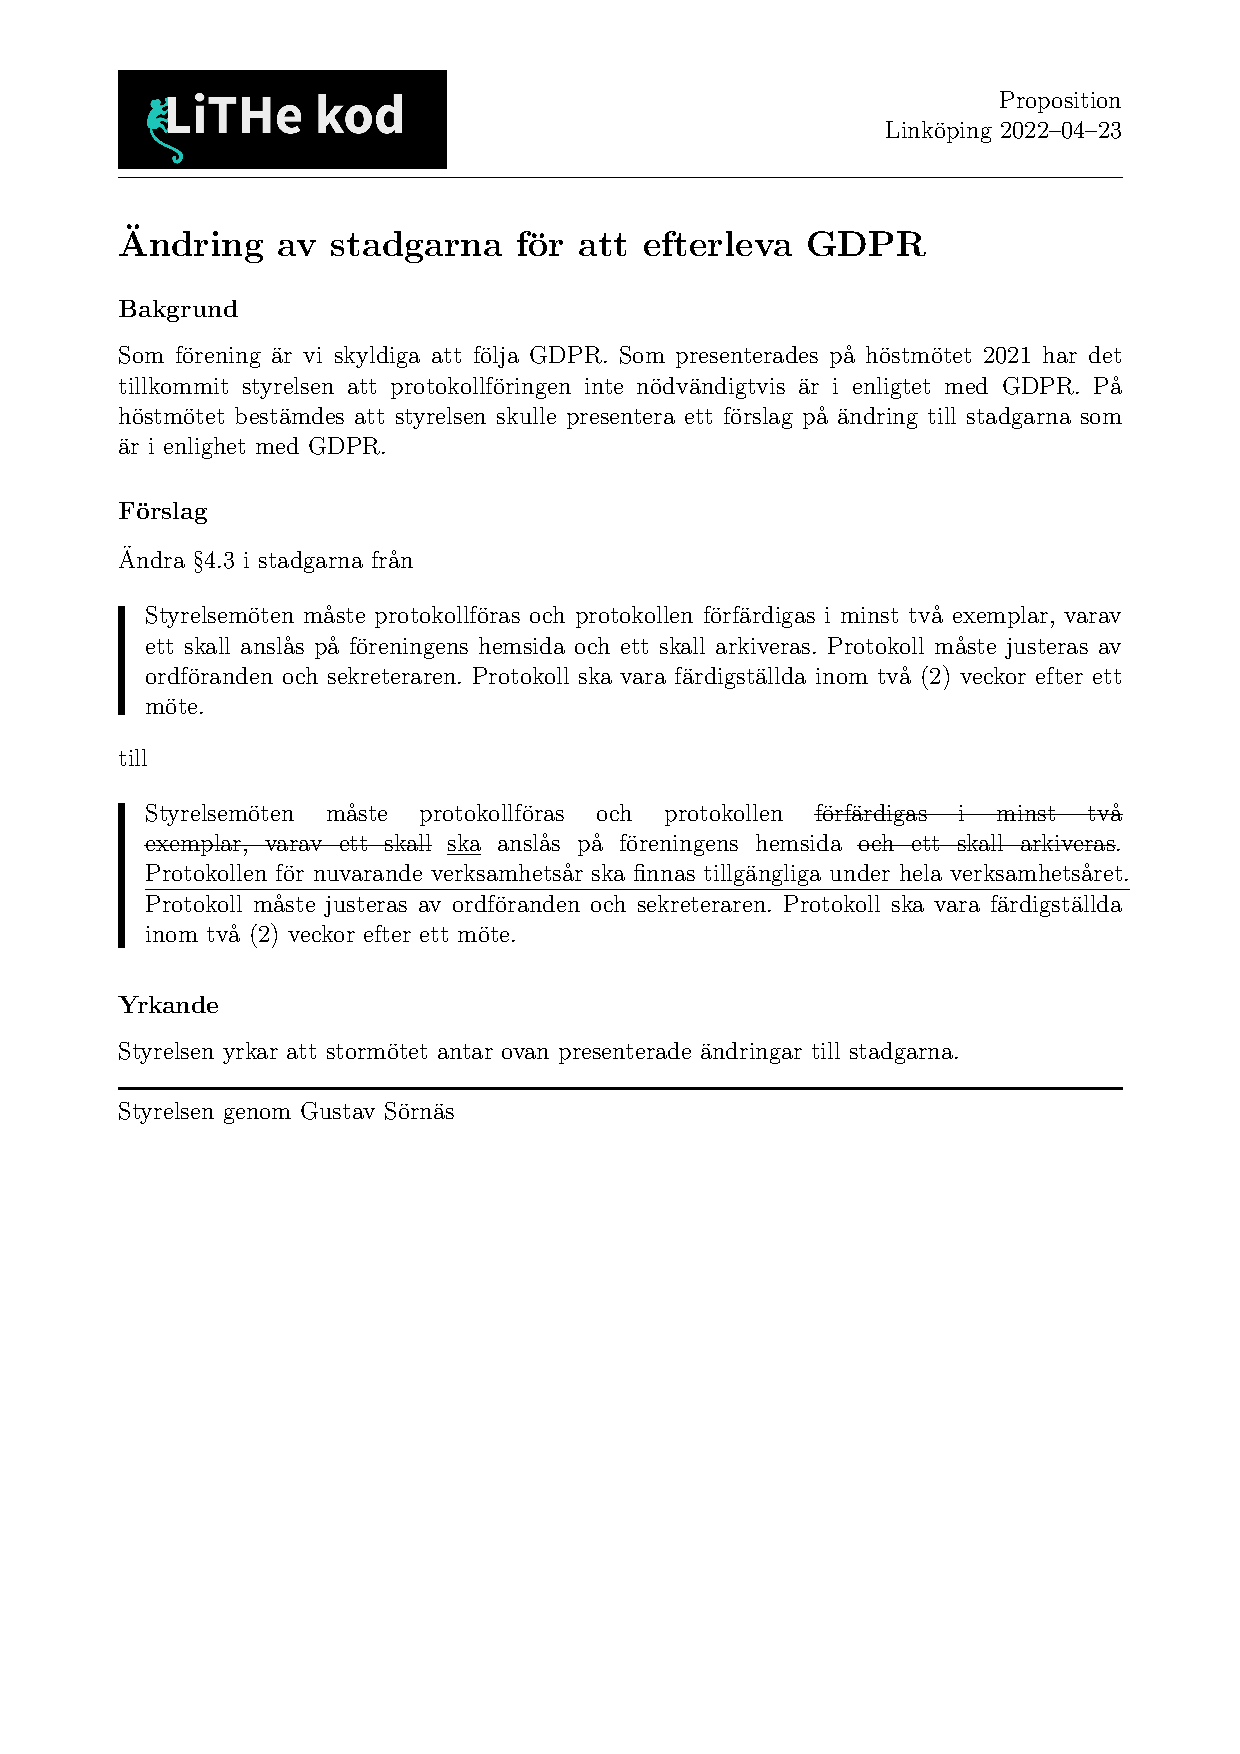
\includepdf[pages=-,pagecommand={},width=\textwidth,frame=true]{220510-bilaga1-gdpr.pdf}
\clearpage
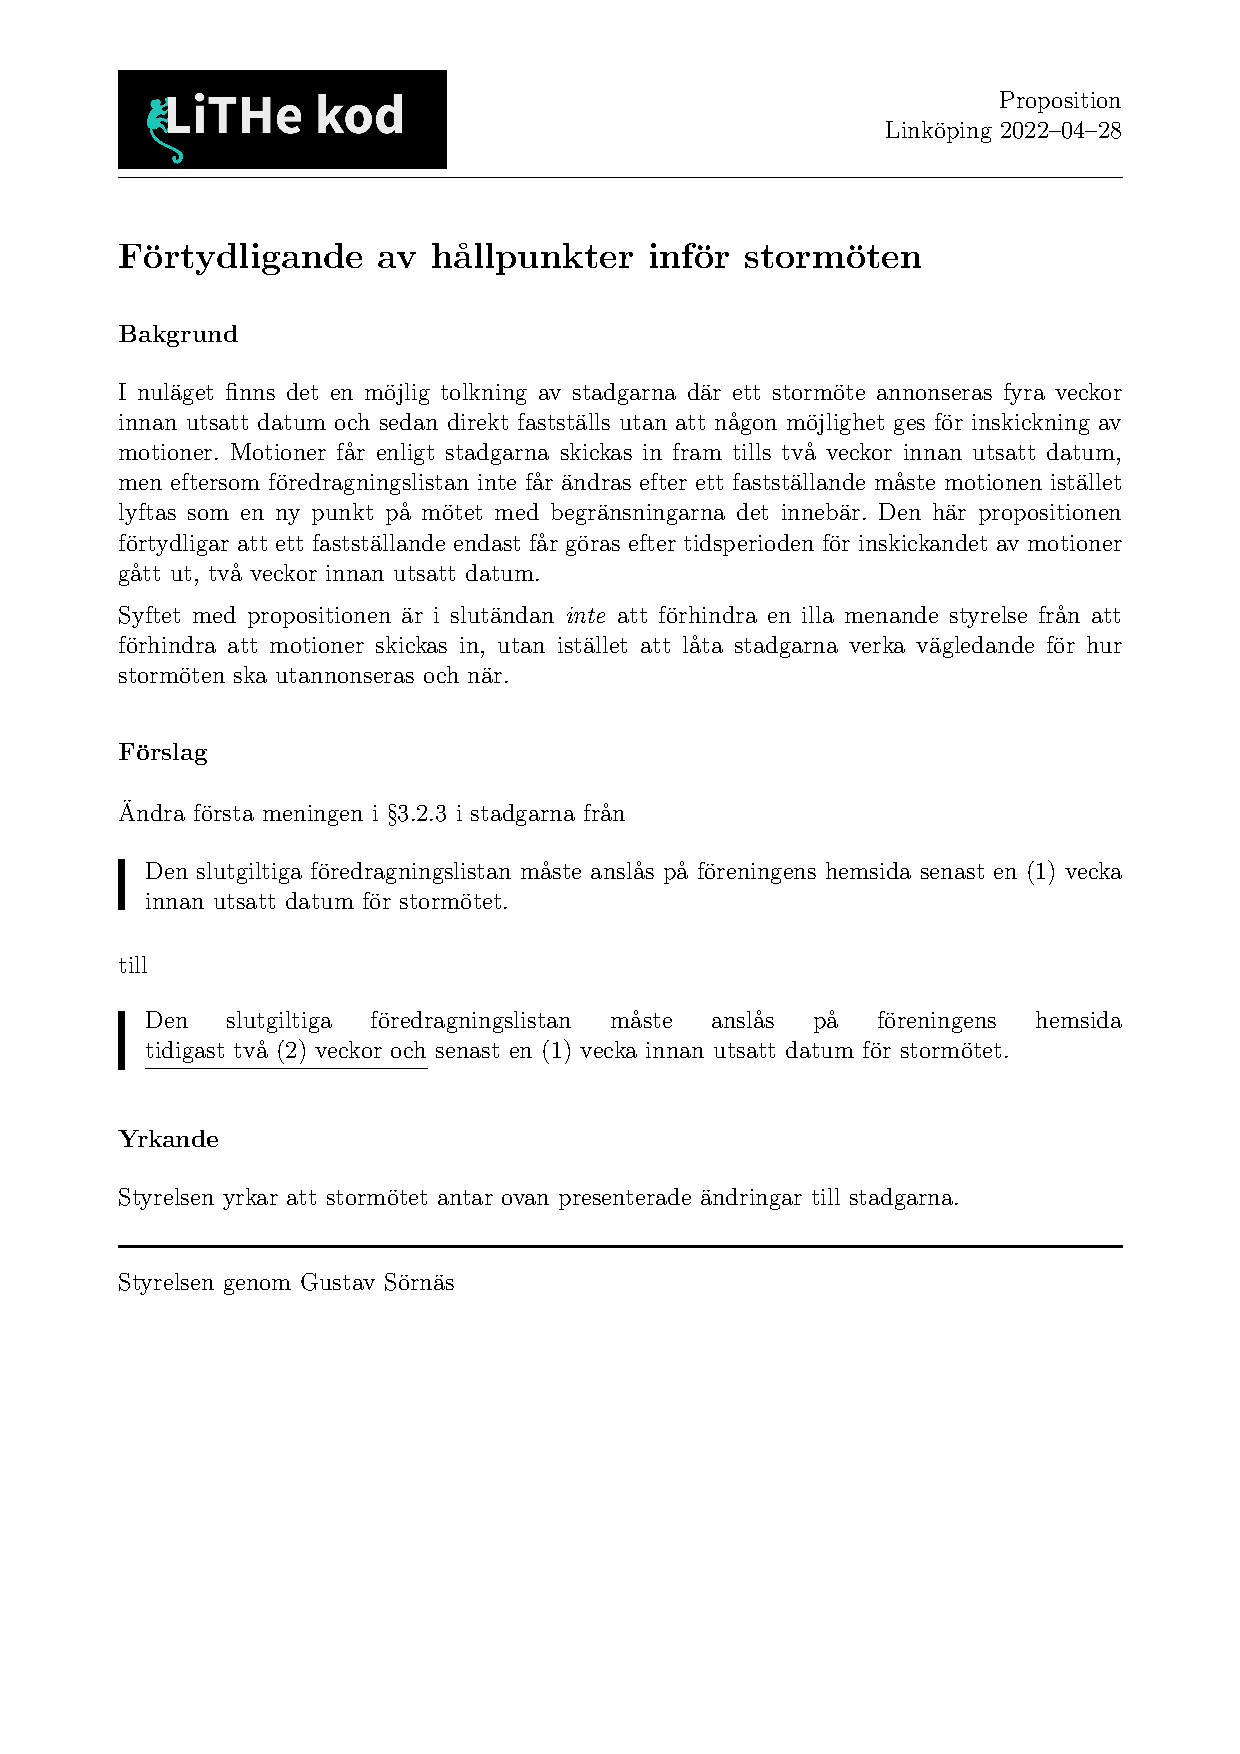
\includepdf[pages=-,pagecommand={},width=\textwidth,frame=true]{220510-bilaga2-stormotestider.pdf}
\clearpage
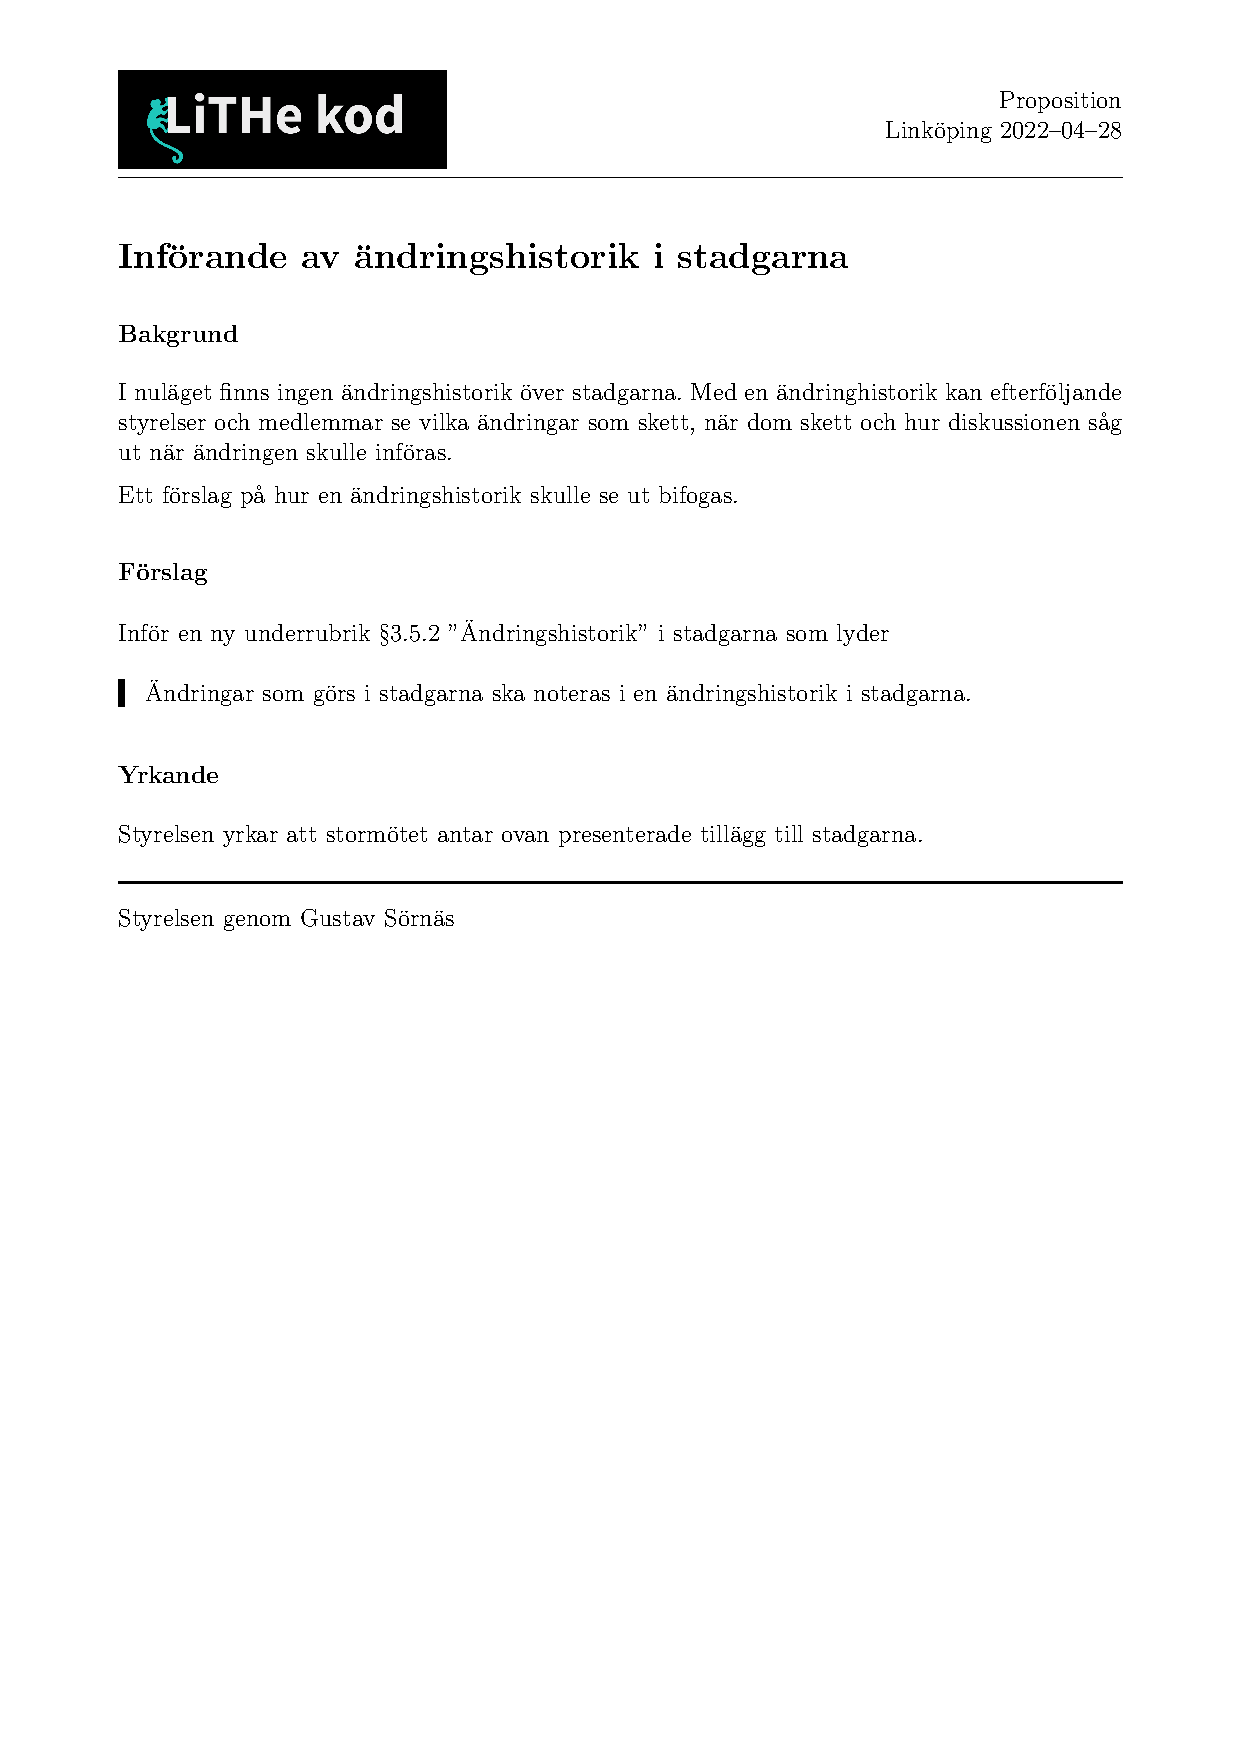
\includepdf[pages=-,pagecommand={},width=\textwidth,frame=true]{220510-bilaga3-historik.pdf}

\end{document}
